\section{Graphen}
\authors{Jakob Gierschmann und Annika Dunkel}

\subsection{Was sind Graphen?}
\begin{figure}
\centering
	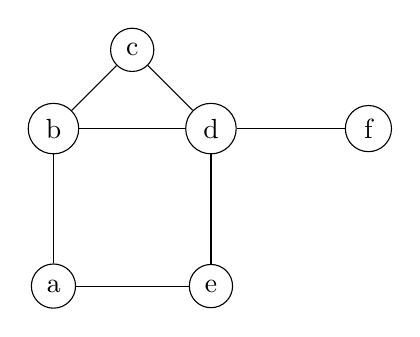
\begin{tikzpicture}
	\node[draw, circle](a) at (1,0){a};
	\node[draw, circle](b) at (1,2){b};
	\node[draw, circle](c) at (2,3){c};
	\node[draw, circle](d) at (3,2){d};
	\node[draw, circle](e) at (3,0){e};
	\node[draw, circle](f) at (5,2){f};
	\draw (a) -- (b);
	\draw (b) -- (d);
	\draw (c) -- (b);
	\draw (c) -- (d);
	\draw (d) -- (f);
	\draw (d) -- (e);
	\draw (a) -- (e);
	\end{tikzpicture}
	\caption{Ein Graph}
	\label{einfuehrungsgraph}
\end{figure}

Ein \wichtig{Graph} besteht aus \wichtig{Knoten} und \wichtig{Kanten}.  
Abb. \ref{einfuehrungsgraph} zeigt ein einfaches Beispiel für einen Graphen.


\begin{df}
Ein Graph ist ein Tupel $G = (V,E)$ aus einer endlichen Knotenmenge $V$ und einer Kantenmenge $E \subseteq \{e \in 2^{V}\mid |e| = 2\}$.
\end{df}

\subsection{Geschichte der Graphentheorie}
\textit{Leonhard Euler} (1707--1783) wird im Allgemeinen als Begründer der Graphentheorie bezeichnet. Er befasste sich mit Problemstellungen wie dem \wichtig{Königsberger Brückenproblem}.
Auch wenn er bereits die ersten Konzepte der Graphentheorie auf aufstellte, entwickelte sich die Graphentheorie in den folgenden 100 Jahren kaum weiter. 
Erst \textit{Gustav Robert Kirchhoff} (1824--1887), der elektrische Ströme mithilfe der Graphentheorie darstellte, ermöglichte dadurch den nächsten großen Durchbruch.
Schließlich brachte \textit{Arthur Cayley} (1821--1895)  die Strukturformeln von chemischen Molekülen in die Graphentheorie ein. Außerdem stellte er den \wichtig{Vierfarbensatz} auf.
Ab 1945 machte die Graphentheorie aufgrund der rasanten Computerentwicklung noch größere Fortschritte.

\subsection{Teilgraphen}
	Ein Teilgraph $G'$ besteht aus einem Teil der Knoten und Kanten eines übergeordneten Graphen $G$.
	\begin{df}
	Ein Graph $ G' = (V', E')$ ist ein Teilgraph von $G = (V, E)$, wenn $V' \subseteq V$ und $E' \subseteq E$, sodass für alle $e = \{v_1, v_2\} \in E'$ auch $v_1, v_2 \in V'$.
	\end{df}
	\begin{df}
	Ein Teilgraph $ G' = (V', E')$ von $G = (V, E)$ heißt von $V'$ induzierter Teilgraph, wenn jede Kante $e \in E$ , die zwischen Knoten $v'_1,v'_2 \in V'$ verläuft, auch in $E'$ vorhanden ist.
	\end{df}

\subsection{Verbindungen}
Graphen haben einige wichtige Eigenschaften, die wir im Folgenden beschreiben und definieren wollen.



\begin{df}
Ein Weg der Länge n ist eine Folge von Knoten $v_0,v_1, v_2, \dotsc, v_n \in V$, sodass Kanten $e = \{v_{i-1},v_i\} \in E$ für $ 1 \leq i \leq n$ existieren.
\end{df}

\begin{df}
Ein Pfad ist ein Weg, bei dem alle Knoten paarweise verschieden sind.
$v_0$ heißt Startknoten und $v_n$ heißt Zielknoten.
\end{df}

\begin{df}
Ein Graph $G = (V,E)$ heißt zusammenhängend, wenn zu je zwei Knoten $v_1, v_2 \in V$ein Pfad von $v_1$ nach $v_2$ existiert.
\end{df}

\begin{df}
Die maximalen zusammenhängenden Teilgraphen heißen Zusammenhangskomponenten.
\end{df}

\subsection{Variationen}

Neben den gewöhnlichen Graphen gibt es einige \wichtig{Variationen}, die in der Regel ausdrücklich als solche gekennzeichnet werden.


\begin{itemize}
\item \wichtig{Multigraphen} Ein  Multigraph lässt mehrere Kanten statt nur einer Kante zwischen zwei Knoten zu.
\item \wichtig{Gerichteter Graphen} Bei einem gerichteten Graphen sind die Kanten keine Mengen, sondern Tupel. Die Knoten, die sie verbinden haben also eine Reihenfolge und somit hat die Kante eine feste Richtung.
\item \wichtig{Graphen mit Schleifen}  Wenn ein Knoten durch eine Kante mit sich selbs verbundn ist, ist diese Kante eine Schleife. In Graphen, die Schleifen zulassen, ist also ist $|e| = 1$ zulässig.
\item \wichtig{Unendliche Graphen} Wenn Graphen eine unendliche Anzahl von Knoten $V$ und/oder Kanten  $E$ haben, werden sie unendliche Graphen genannt.
\end{itemize}

\subsection{Spezielle Graphen}
In der Graphentheorie gibt es spezielle Graphen, die besondere Eigenschaften haben. Einige von ihnen nennen wir kurz, um uns später auf sie beziehen zu können.


\begin{figure}
	\centering
	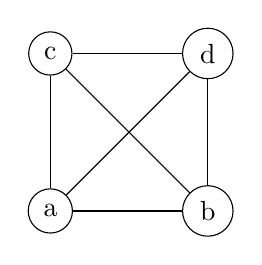
\begin{tikzpicture}
	\node[draw, circle](a) at (0,0){a};
	\node[draw, circle](b) at (2,0){b};
	\node[draw, circle](c) at (0,2){c};
	\node[draw, circle](d) at (2,2){d};
	\draw(a) -- (b);
	\draw(a) -- (c);
	\draw(a) -- (d);
	\draw(b) -- (c);
	\draw(b) -- (d);
	\draw(c) -- (d);
	\end{tikzpicture}
	
	\caption{Der Graph $K_4$}
	\label{k4}
\end{figure}

\begin{figure}
	\centering
	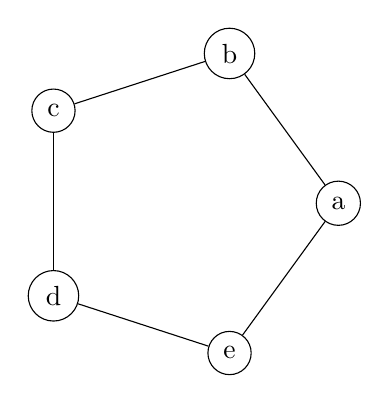
\begin{tikzpicture}
	\node[draw, circle](a) at (0.0:2){a};
	\node[draw, circle](b) at (72.0:2){b};
	\node[draw, circle](c) at (144.0:2){c};
	\node[draw, circle](d) at (216.0:2){d};
	\node[draw, circle](e) at (288.0:2){e};
	\draw(a) -- (b);
	\draw(b) -- (c);
	\draw(c) -- (d);
	\draw(d) -- (e);
	\draw(e) -- (a);
	\end{tikzpicture}
	\caption{Der Graph $C_5$}
	\label{c5}
\end{figure}

\begin{figure}
	\centering
	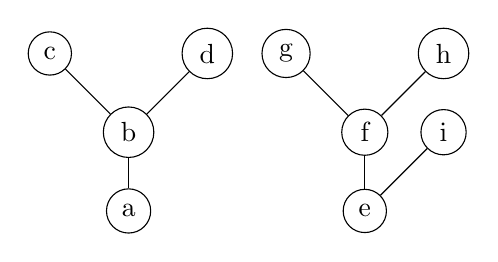
\begin{tikzpicture}
	\node[draw, circle](a) at (1,0){a};
	\node[draw, circle](b) at (1,1){b};
	\node[draw, circle](c) at (0,2){c};
	\node[draw, circle](d) at (2,2){d};
	\node[draw, circle](e) at (4,0){e};
	\node[draw, circle](f) at (4,1){f};
	\node[draw, circle](g) at (3,2){g};
	\node[draw, circle](h) at (5,2){h};
	\node[draw, circle](i) at (5,1){i};
	\draw(a) -- (b);
	\draw(b) -- (c);
	\draw(b) -- (d);
	\draw(e) -- (f);
	\draw(f) -- (g);
	\draw(f) -- (h);
	\draw(e) -- (i);

	\end{tikzpicture}
	\caption{Ein Wald aus zwei Bäumen}
	\label{wood}
\end{figure}
\begin{df}
Ein vollständiger Graph $K_n$ ist ein Graph $G = (V,E)$ mit $n$ Knoten, bei dem je zwei Knoten $v,w \in V$ durch eine Kante $ e = \{v,w\} $ verbunden sind.
\end{df}
Ein Beispiel für einen vollständigen Graphen ist der Graph $K_4$ in Abb. \ref{k4}.
\begin{df}
Ist $v_0,v_1,\dotsc,v_n$ ein Pfad und existiert $e_0 = \{v_n, v_o\}$ so ist $v_0, v_1, \dotsc, v_n$ ein Kreis. Einen Kreis mit $n$ Knoten nennen wir $C_n$.
\end{df}
Ein Beispiel für einen Kreis ist der Graph $C_5$ in Abb. \ref{c5}.
\begin{df}
Ein Wald ist ein Graph ohne Kreise. Die Zusammenhangskomponenten heißen Bäume.
\end{df}
Abb. \ref{wood} zeigt ein Beispiel für einen Wald.





\subsection{Wichtige Messgrößen}
Es gibt in Graphen einige Meßgrößen, die wir durch Funktionen oder Variablen angeben können. Einige seien hier kurz definiert.\\

Der Grad eines Knotens ist ein Beispiel für eine lokale Messgröße, da wir ihn beschreiben können, ohne den ganzen Graphen zu betrachten.
\begin{df}
Sei $v \in V$ ein Knoten.
Der Grad von $v$, geschrieben $d(v)$, ist die Anzahl an Kanten, die $v$ enthalten.
\begin{center}
$d(v) := |\{e \in E \mid v \in e\}|$
\end{center}
\end{df}

\begin{df}
Das Minimum aller Grade der Knoten $v \in V$ wird mit $\delta$ bezeichnet, das Maximum mit $\Delta$.
\end{df}

\begin{fakt}
Die Summe $\sum\limits_{v\in V}d(v)$ ist gerade und $|E|  = \frac{1}{2}\sum\limits_{v\in V}d(v)$.
\begin{proof}
Jede Kante verbindet zwei Knoten, also erhöht jede Kante die Summe aller Grade um 2.
\end{proof}
\end{fakt}

Mit den gerade definierten Eigenschaften von Graphen können wir eine weitere Funktion einführen, die wir benutzen können, um Knoten besser differenzieren zu können.

\begin{df}
Der Abstand $d(v,v')$ zwischen zwei Knoten $v,v' \in V$ ist die Länge des kürzesten Pfades von $v$ nach $v'$. Gibt es keinen solchen Pfad, so setzen wir $d(v,v') = \infty$.
\end{df}



%\subsection{Kreise und Bäume}




